%%======================================================================
%%  Chapitre 3 : Conception du projet
%%======================================================================
\chapter{Conception du projet}

Ce chapitre présente la phase de conception de la plateforme éducative. Nous y décrivons l'architecture globale du système, le diagramme de classes, les cas d'utilisation de chaque acteur, ainsi que les diagrammes de séquence des processus clés.

%%======================================================================
\section{Architecture globale du système}

\subsection{Architecture 3-tiers (Client -- Serveur -- Base de données)}

La plateforme \textit{EduPlatform} adopte une \textbf{architecture 3-tiers} classique qui sépare l'application en trois couches distinctes :

\begin{enumerate}
    \item \textbf{Couche Présentation (Client)} : l'application React/TypeScript qui s'exécute dans le navigateur de l'utilisateur. Elle communique avec le serveur via des requêtes HTTP (API REST) ;
    \item \textbf{Couche Logique Métier (Serveur)} : l'application Spring Boot qui reçoit les requêtes HTTP, exécute la logique métier et retourne des réponses JSON ;
    \item \textbf{Couche Données (Base de données)} : la base de données MySQL (ou H2 en développement) qui stocke l'ensemble des données persistantes.
\end{enumerate}

\begin{figure}[H]
\centering
\begin{tikzpicture}[
    box/.style={draw, rounded corners=8pt, minimum width=12cm, minimum height=2cm, 
                text centered, font=\sffamily\bfseries},
    arrow/.style={-{Stealth[length=3mm]}, thick, color=NavyBlue}
]

% Client
\node[box, fill=blue!10] (client) at (0,6) {
    \begin{tabular}{c}
    \textcolor{NavyBlue}{Couche Présentation (Client)} \\
    \small\normalfont React + TypeScript + Vite (port 5174)
    \end{tabular}
};

% Serveur
\node[box, fill=green!10] (server) at (0,3) {
    \begin{tabular}{c}
    \textcolor{ForestGreen}{Couche Logique Métier (Serveur)} \\
    \small\normalfont Spring Boot + JPA/Hibernate (port 8081)
    \end{tabular}
};

% BDD
\node[box, fill=orange!10] (db) at (0,0) {
    \begin{tabular}{c}
    \textcolor{BurntOrange}{Couche Données (Base de données)} \\
    \small\normalfont MySQL 8.0 / H2 — 23 tables
    \end{tabular}
};

% Flèches
\draw[arrow] (client.south) -- node[right, font=\small] {HTTP REST (JSON)} (server.north);
\draw[arrow] (server.south) -- node[right, font=\small] {JDBC / JPA} (db.north);

\end{tikzpicture}
\caption{Architecture 3-tiers de la plateforme}
\label{fig:archi_3tiers}
\end{figure}

\subsection{Pattern MVC (Model -- View -- Controller)}

Au sein du backend Spring Boot, nous appliquons le pattern \textbf{MVC} adapté aux API REST. Chaque requête traverse quatre couches successives :

\begin{figure}[H]
\centering
\begin{tikzpicture}[
    layer/.style={draw, rounded corners=5pt, minimum width=3.5cm, minimum height=1.5cm, 
                  text centered, font=\sffamily\small},
    arrow/.style={-{Stealth[length=2.5mm]}, thick}
]

\node[layer, fill=blue!15] (ctrl) at (0,0) {Controller\\{\tiny (28 contrôleurs)}};
\node[layer, fill=green!15] (svc) at (4.5,0) {Service\\{\tiny (27 services)}};
\node[layer, fill=orange!15] (repo) at (9,0) {Repository\\{\tiny (25 interfaces)}};
\node[layer, fill=red!10] (db) at (13.5,0) {Database\\{\tiny (23 tables)}};

\draw[arrow] (ctrl) -- node[above, font=\tiny] {appel} (svc);
\draw[arrow] (svc) -- node[above, font=\tiny] {requête} (repo);
\draw[arrow] (repo) -- node[above, font=\tiny] {SQL} (db);

\end{tikzpicture}
\caption{Flux de données dans le pattern MVC}
\label{fig:mvc_flow}
\end{figure}

\begin{table}[H]
\centering
\caption{Statistiques de l'architecture backend}
\label{tab:archi_stats}
\begin{tabular}{lc}
\toprule
\textbf{Composant} & \textbf{Nombre} \\
\midrule
Entités JPA (Model) & 25 \\
Repositories (JPA) & 25 \\
Services (Logique métier) & 27 \\
Contrôleurs REST & 28 \\
Endpoints API & 90+ \\
DTOs (transfert de données) & 10+ \\
Tables en base & 23 \\
\bottomrule
\end{tabular}
\end{table}

%%======================================================================
\section{Diagramme de classes}

\subsection{Hiérarchie d'héritage (User $\rightarrow$ Admin, Enseignant, Étudiant)}

La modélisation des utilisateurs repose sur un \textbf{héritage de type SINGLE\_TABLE}. La classe abstraite \texttt{User} contient les attributs communs, et chaque rôle est représenté par une sous-classe avec ses attributs spécifiques.

\begin{figure}[H]
\centering
\begin{tikzpicture}[
    class/.style={draw, rectangle, rounded corners=3pt, minimum width=5cm,
                  font=\small\ttfamily, inner sep=6pt},
    inherit/.style={-{Triangle[length=3mm, open]}, thick}
]

% User
\node[class, fill=blue!10] (user) at (0,0) {
    \begin{tabular}{l}
    \textbf{User} (abstract) \\
    \hline
    id : Long \\
    email : String (unique) \\
    password : String \\
    firstName : String \\
    lastName : String \\
    phoneNumber : String \\
    address : String \\
    profilePicture : String \\
    isActive : Boolean \\
    createdAt : LocalDateTime \\
    updatedAt : LocalDateTime \\
    \hline
    getRole() : Role
    \end{tabular}
};

% Admin
\node[class, fill=red!10] (admin) at (-6,-6) {
    \begin{tabular}{l}
    \textbf{Admin} \\
    \hline
    (pas de champs\\supplémentaires) \\
    \hline
    Gère le système
    \end{tabular}
};

% Enseignant
\node[class, fill=green!10] (ens) at (0,-6) {
    \begin{tabular}{l}
    \textbf{Enseignant} \\
    \hline
    specialite : String \\
    \hline
    departement : Departement \\
    cours : List<Cours> \\
    absences : List<Absence>
    \end{tabular}
};

% Etudiant
\node[class, fill=orange!10] (etu) at (6,-6) {
    \begin{tabular}{l}
    \textbf{Etudiant} \\
    \hline
    niveau : String \\
    \hline
    groupe : Groupe \\
    departement : Departement \\
    cours : List<Cours> \\
    notes : List<Note> \\
    absences : List<Absence>
    \end{tabular}
};

% Flèches d'héritage
\draw[inherit] (admin.north) -- (user.south west);
\draw[inherit] (ens.north) -- (user.south);
\draw[inherit] (etu.north) -- (user.south east);

\end{tikzpicture}
\caption{Hiérarchie d'héritage des utilisateurs}
\label{fig:class_user}
\end{figure}

\subsection{Entités principales}

Le système comporte \textbf{25 entités JPA} organisées autour des domaines fonctionnels suivants :

\begin{table}[H]
\centering
\caption{Liste des entités du système}
\label{tab:entites}
\begin{tabularx}{\textwidth}{llX}
\toprule
\textbf{Domaine} & \textbf{Entité} & \textbf{Description} \\
\midrule
\multirow{4}{*}{Utilisateurs} 
 & User & Classe de base (abstraite) avec les attributs communs \\
 & Admin & Administrateur du système \\
 & Enseignant & Professeur avec spécialité et département \\
 & Etudiant & Étudiant avec niveau et groupe \\
\midrule
\multirow{3}{*}{Organisation}
 & Departement & Unité organisationnelle (ex: Informatique) \\
 & Groupe & Groupe d'étudiants (A, B, C…) \\
 & Classe & Classe d'enseignement avec niveau \\
\midrule
\multirow{3}{*}{Pédagogie}
 & Cours & Module d'enseignement avec coefficient et volume horaire \\
 & Matiere & Matière rattachée à un cours \\
 & EmploiDuTemps & Emploi du temps (jour, heure, salle) \\
\midrule
\multirow{3}{*}{Évaluations}
 & Devoir & Travail assigné avec date limite \\
 & Soumission & Réponse à un devoir (fichier + contenu) \\
 & Evaluation & Épreuve/examen planifié \\
 & Note & Note attribuée à un étudiant par matière \\
\midrule
\multirow{2}{*}{Absences}
 & Absence & Enregistrement d'absence (statut : justifiée/non) \\
 & Justification & Justification d'absence avec document \\
\midrule
\multirow{3}{*}{Administration}
 & Demande & Demande administrative (attestation, etc.) \\
 & Demande\_Stage & Demande spécifique de stage \\
 & Reclamation & Réclamation générale \\
 & ReclamationNote & Réclamation de note (workflow multi-étapes) \\
\midrule
\multirow{2}{*}{Communication}
 & Notification & Notification avec workflow d'approbation \\
 & Commentaire & Commentaire avec suppression logique \\
\midrule
Autre
 & Inscription & Inscription d'un étudiant à une classe \\
 & Projet & Projet collaboratif enseignant-étudiants \\
\bottomrule
\end{tabularx}
\end{table}

\subsection{Relations entre entités}

Les relations entre entités sont de trois types : \texttt{OneToMany}, \texttt{ManyToOne} et \texttt{ManyToMany}.

\begin{figure}[H]
\centering
\begin{tikzpicture}[
    entity/.style={draw, rectangle, rounded corners=3pt, minimum width=3cm,
                   minimum height=1cm, text centered, font=\small\sffamily\bfseries,
                   fill=#1!15},
    rel/.style={-{Stealth[length=2mm]}, thick, color=gray!70},
    relm/.style={thick, color=NavyBlue, dashed}
]

% Entités principales
\node[entity=blue] (dep) at (0,8) {Département};
\node[entity=green] (ens) at (-4,6) {Enseignant};
\node[entity=orange] (etu) at (4,6) {Étudiant};
\node[entity=purple] (grp) at (8,8) {Groupe};
\node[entity=teal] (cours) at (0,4) {Cours};
\node[entity=red] (dev) at (-4,2) {Devoir};
\node[entity=cyan] (soum) at (-4,0) {Soumission};
\node[entity=brown] (abs) at (4,2) {Absence};
\node[entity=olive] (just) at (8,2) {Justification};
\node[entity=violet] (note) at (4,0) {Note};
\node[entity=magenta] (mat) at (0,0) {Matière};
\node[entity=gray] (edt) at (0,2) {EmploiDuTemps};
\node[entity=pink] (notif) at (8,5) {Notification};
\node[entity=lime] (dem) at (-6,4) {Demande};

% Relations 1:N
\draw[rel] (dep) -- node[left, font=\tiny] {1:N} (ens);
\draw[rel] (dep) -- node[right, font=\tiny] {1:N} (etu);
\draw[rel] (dep) -- node[left, font=\tiny] {1:N} (cours);
\draw[rel] (grp) -- node[right, font=\tiny] {1:N} (etu);
\draw[rel] (ens) -- node[left, font=\tiny] {1:N} (cours);
\draw[rel] (cours) -- node[left, font=\tiny] {1:N} (dev);
\draw[rel] (dev) -- node[left, font=\tiny] {1:N} (soum);
\draw[rel] (cours) -- node[left, font=\tiny] {1:N} (abs);
\draw[rel] (abs) -- node[above, font=\tiny] {1:N} (just);
\draw[rel] (cours) -- node[right, font=\tiny] {1:N} (edt);
\draw[rel] (cours) -- node[right, font=\tiny] {1:N} (mat);
\draw[rel] (mat) -- node[right, font=\tiny] {1:N} (note);

% Relations M:N (pointillés)
\draw[relm] (cours) -- node[above, font=\tiny, color=NavyBlue] {N:M} (etu);

\end{tikzpicture}
\caption{Relations entre les entités principales}
\label{fig:relations}
\end{figure}

%%======================================================================
\section{Diagrammes de cas d'utilisation}

\subsection{Cas d'utilisation de l'Administrateur}

L'administrateur dispose des privilèges les plus étendus sur la plateforme.

\begin{figure}[H]
\centering
\begin{tikzpicture}[
    uc/.style={draw, ellipse, minimum width=3.5cm, minimum height=1cm, 
               text centered, font=\small, fill=red!5},
    actor/.style={font=\small\bfseries}
]

% Acteur
\node[actor] (admin) at (-5,4) {Administrateur};
\draw (-5,3.5) circle (0.3);
\draw (-5,3.2) -- (-5,2.5);
\draw (-5.4,2.9) -- (-4.6,2.9);
\draw (-5,2.5) -- (-5.3,1.9);
\draw (-5,2.5) -- (-4.7,1.9);

% Cas d'utilisation
\node[uc] (uc1) at (2,7) {Gérer les utilisateurs};
\node[uc] (uc2) at (2,5.5) {Gérer les départements};
\node[uc] (uc3) at (2,4) {Traiter les demandes};
\node[uc] (uc4) at (2,2.5) {Superviser les absences};
\node[uc] (uc5) at (2,1) {Consulter les justifications};
\node[uc] (uc6) at (2,-0.5) {Gérer les soumissions};
\node[uc] (uc7) at (2,-2) {Consulter les notes};
\node[uc] (uc8) at (2,-3.5) {Traiter les réclamations};
\node[uc] (uc9) at (2,-5) {Envoyer des notifications};

% Liens
\foreach \i in {1,...,9}
    \draw[-] (-4.7,3) -- (uc\i);

% Cadre système
\draw[dashed, rounded corners=10pt] (-1,-6) rectangle (5.5,8);
\node[font=\small\itshape] at (2.25,8.3) {Système EduPlatform};

\end{tikzpicture}
\caption{Diagramme de cas d'utilisation — Administrateur}
\label{fig:uc_admin}
\end{figure}

\begin{table}[H]
\centering
\caption{Description textuelle des cas d'utilisation — Administrateur}
\label{tab:uc_admin}
\begin{tabularx}{\textwidth}{lX}
\toprule
\textbf{Cas d'utilisation} & \textbf{Description} \\
\midrule
Gérer les utilisateurs & CRUD complet sur les comptes Admin, Enseignant et Étudiant (création, modification, activation/désactivation, suppression) \\
Gérer les départements & Créer, modifier et supprimer les départements et groupes \\
Traiter les demandes & Valider ou rejeter les demandes administratives et les demandes de stage \\
Superviser les absences & Consulter toutes les absences par classe et par cours \\
Consulter les justifications & Examiner les justifications soumises et les accepter/refuser \\
Gérer les soumissions & Consulter et superviser l'ensemble des soumissions de devoirs \\
Consulter les notes & Visualiser les notes de tous les étudiants \\
Traiter les réclamations & Traiter les réclamations générales et transférer les réclamations de notes aux enseignants concernés \\
Envoyer des notifications & Envoyer des notifications ciblées ou diffuser des annonces à un rôle entier \\
\bottomrule
\end{tabularx}
\end{table}

\subsection{Cas d'utilisation de l'Enseignant}

\begin{figure}[H]
\centering
\begin{tikzpicture}[
    uc/.style={draw, ellipse, minimum width=3.5cm, minimum height=1cm, 
               text centered, font=\small, fill=green!5},
    actor/.style={font=\small\bfseries}
]

\node[actor] (ens) at (-5,3) {Enseignant};
\draw (-5,2.5) circle (0.3);
\draw (-5,2.2) -- (-5,1.5);
\draw (-5.4,1.9) -- (-4.6,1.9);
\draw (-5,1.5) -- (-5.3,0.9);
\draw (-5,1.5) -- (-4.7,0.9);

\node[uc] (uc1) at (2,5.5) {Gérer ses cours};
\node[uc] (uc2) at (2,4) {Créer des devoirs};
\node[uc] (uc3) at (2,2.5) {Évaluer les soumissions};
\node[uc] (uc4) at (2,1) {Gérer les évaluations};
\node[uc] (uc5) at (2,-0.5) {Marquer les absences};
\node[uc] (uc6) at (2,-2) {Consulter l'emploi du temps};
\node[uc] (uc7) at (2,-3.5) {Traiter les réclamations de notes};
\node[uc] (uc8) at (2,-5) {Envoyer des notifications};

\foreach \i in {1,...,8}
    \draw[-] (-4.7,2) -- (uc\i);

\draw[dashed, rounded corners=10pt] (-1,-6) rectangle (5.5,6.5);
\node[font=\small\itshape] at (2.25,6.8) {Système EduPlatform};

\end{tikzpicture}
\caption{Diagramme de cas d'utilisation — Enseignant}
\label{fig:uc_enseignant}
\end{figure}

\subsection{Cas d'utilisation de l'Étudiant}

\begin{figure}[H]
\centering
\begin{tikzpicture}[
    uc/.style={draw, ellipse, minimum width=3.5cm, minimum height=1cm, 
               text centered, font=\small, fill=orange!5},
    actor/.style={font=\small\bfseries}
]

\node[actor] (etu) at (-5,3) {Étudiant};
\draw (-5,2.5) circle (0.3);
\draw (-5,2.2) -- (-5,1.5);
\draw (-5.4,1.9) -- (-4.6,1.9);
\draw (-5,1.5) -- (-5.3,0.9);
\draw (-5,1.5) -- (-4.7,0.9);

\node[uc] (uc1) at (2,6.5) {Consulter les cours};
\node[uc] (uc2) at (2,5) {Soumettre un devoir};
\node[uc] (uc3) at (2,3.5) {Consulter les notes};
\node[uc] (uc4) at (2,2) {Consulter les absences};
\node[uc] (uc5) at (2,0.5) {Déposer une justification};
\node[uc] (uc6) at (2,-1) {Envoyer une demande};
\node[uc] (uc7) at (2,-2.5) {Demander un stage};
\node[uc] (uc8) at (2,-4) {Déposer une réclamation};
\node[uc] (uc9) at (2,-5.5) {Consulter l'emploi du temps};
\node[uc] (uc10) at (2,-7) {Consulter les notifications};

\foreach \i in {1,...,10}
    \draw[-] (-4.7,2) -- (uc\i);

\draw[dashed, rounded corners=10pt] (-1,-8) rectangle (5.5,7.5);
\node[font=\small\itshape] at (2.25,7.8) {Système EduPlatform};

\end{tikzpicture}
\caption{Diagramme de cas d'utilisation — Étudiant}
\label{fig:uc_etudiant}
\end{figure}

%%======================================================================
\section{Diagrammes de séquence}

\subsection{Diagramme de séquence : Authentification (Login)}

Le processus d'authentification se déroule en plusieurs étapes : l'utilisateur saisit ses identifiants, le frontend contacte le backend via l'API REST, et le backend vérifie les informations dans la base de données.

\begin{figure}[H]
\centering
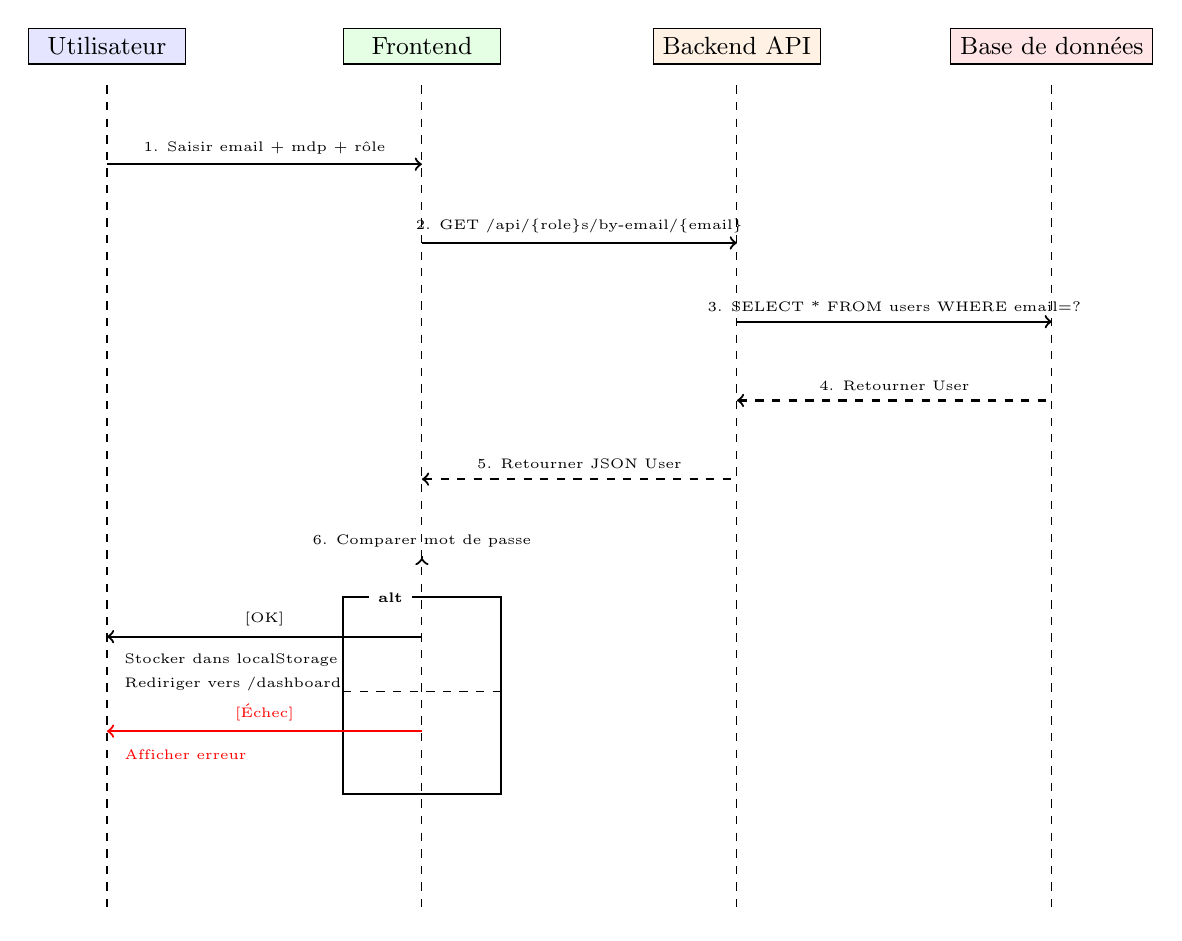
\begin{tikzpicture}[font=\small]

% Participants
\node[draw, rectangle, fill=blue!10, minimum width=2cm] (user) at (0,0) {Utilisateur};
\node[draw, rectangle, fill=green!10, minimum width=2cm] (front) at (4,0) {Frontend};
\node[draw, rectangle, fill=orange!10, minimum width=2cm] (back) at (8,0) {Backend API};
\node[draw, rectangle, fill=red!10, minimum width=2cm] (db) at (12,0) {Base de données};

% Lignes de vie
\draw[dashed] (0,-0.5) -- (0,-11);
\draw[dashed] (4,-0.5) -- (4,-11);
\draw[dashed] (8,-0.5) -- (8,-11);
\draw[dashed] (12,-0.5) -- (12,-11);

% Messages
\draw[->, thick] (0,-1.5) -- node[above, font=\tiny] {1. Saisir email + mdp + rôle} (4,-1.5);
\draw[->, thick] (4,-2.5) -- node[above, font=\tiny] {2. GET /api/\{role\}s/by-email/\{email\}} (8,-2.5);
\draw[->, thick] (8,-3.5) -- node[above, font=\tiny] {3. SELECT * FROM users WHERE email=?} (12,-3.5);
\draw[<-, thick, dashed] (8,-4.5) -- node[above, font=\tiny] {4. Retourner User} (12,-4.5);
\draw[<-, thick, dashed] (4,-5.5) -- node[above, font=\tiny] {5. Retourner JSON User} (8,-5.5);
\draw[->, thick] (4,-6.5) -- node[above, font=\tiny] {6. Comparer mot de passe} (4,-6.5);

% Alt box
\draw[thick] (3,-7) rectangle (5,-9.5);
\node[fill=white, font=\tiny\bfseries] at (3.6,-7) {alt};
\draw[dashed] (3,-8.2) -- (5,-8.2);

\draw[->, thick] (4,-7.5) -- node[above, font=\tiny] {[OK]} (0,-7.5);
\node[font=\tiny, right] at (0.1,-7.8) {Stocker dans localStorage};
\node[font=\tiny, right] at (0.1,-8.1) {Rediriger vers /dashboard};

\draw[->, thick, red] (4,-8.7) -- node[above, font=\tiny, red] {[Échec]} (0,-8.7);
\node[font=\tiny, right, red] at (0.1,-9) {Afficher erreur};

\end{tikzpicture}
\caption{Diagramme de séquence — Authentification}
\label{fig:seq_login}
\end{figure}

\textbf{Description du processus :}
\begin{enumerate}[noitemsep]
    \item L'utilisateur saisit son email, son mot de passe et sélectionne son rôle (Admin / Enseignant / Étudiant) ;
    \item Le frontend envoie une requête GET à l'endpoint correspondant au rôle (ex: \texttt{/api/etudiants/by-email/\{email\}}) ;
    \item Le backend interroge la base de données pour trouver l'utilisateur par email ;
    \item Si l'utilisateur existe, ses informations sont retournées au frontend ;
    \item Le frontend compare le mot de passe saisi avec celui retourné ;
    \item En cas de succès, l'utilisateur est stocké dans le \texttt{localStorage} et redirigé vers son tableau de bord. En cas d'échec, un message d'erreur est affiché.
\end{enumerate}

\subsection{Diagramme de séquence : Soumission d'un devoir}

\begin{figure}[H]
\centering
\begin{tikzpicture}[font=\small]

\node[draw, rectangle, fill=orange!10, minimum width=2cm] (etu) at (0,0) {Étudiant};
\node[draw, rectangle, fill=green!10, minimum width=2cm] (front) at (4,0) {Frontend};
\node[draw, rectangle, fill=blue!10, minimum width=2.5cm] (ctrl) at (8.5,0) {SoumissionCtrl};
\node[draw, rectangle, fill=purple!10, minimum width=2.5cm] (svc) at (13,0) {SoumissionSvc};

\draw[dashed] (0,-0.5) -- (0,-10);
\draw[dashed] (4,-0.5) -- (4,-10);
\draw[dashed] (8.5,-0.5) -- (8.5,-10);
\draw[dashed] (13,-0.5) -- (13,-10);

\draw[->, thick] (0,-1.5) -- node[above, font=\tiny] {1. Remplir formulaire + fichier} (4,-1.5);
\draw[->, thick] (4,-2.5) -- node[above, font=\tiny] {2. POST /api/soumissions/submit-file} (8.5,-2.5);
\draw[->, thick] (8.5,-3.5) -- node[above, font=\tiny] {3. submitWithFile(data)} (13,-3.5);
\draw[->, thick] (13,-4.5) -- node[above, font=\tiny, align=center] {4. Sauvegarder fichier\\+ créer Soumission} (13,-4.5);
\draw[<--, thick, dashed] (8.5,-5.5) -- node[above, font=\tiny] {5. Soumission créée} (13,-5.5);
\draw[<--, thick, dashed] (4,-6.5) -- node[above, font=\tiny] {6. ApiResponse (succès)} (8.5,-6.5);
\draw[<--, thick, dashed] (0,-7.5) -- node[above, font=\tiny] {7. Confirmation visuelle} (4,-7.5);

% Notification
\draw[->, thick, NavyBlue] (13,-8.5) -- node[above, font=\tiny, NavyBlue] {8. Notification → Enseignant} (13,-8.5);
\node[font=\tiny, NavyBlue, right] at (9,-9) {Type: DEVOIR\_UPLOAD};

\end{tikzpicture}
\caption{Diagramme de séquence — Soumission d'un devoir}
\label{fig:seq_soumission}
\end{figure}

\subsection{Diagramme de séquence : Gestion des absences}

\begin{figure}[H]
\centering
\begin{tikzpicture}[font=\small]

\node[draw, rectangle, fill=green!10, minimum width=2cm] (ens) at (0,0) {Enseignant};
\node[draw, rectangle, fill=blue!10, minimum width=2cm] (front) at (4,0) {Frontend};
\node[draw, rectangle, fill=orange!10, minimum width=2cm] (back) at (8,0) {Backend};
\node[draw, rectangle, fill=red!10, minimum width=2cm] (db) at (12,0) {Database};

\draw[dashed] (0,-0.5) -- (0,-12);
\draw[dashed] (4,-0.5) -- (4,-12);
\draw[dashed] (8,-0.5) -- (8,-12);
\draw[dashed] (12,-0.5) -- (12,-12);

% Marquage absence
\draw[->, thick] (0,-1.5) -- node[above, font=\tiny] {1. Marquer absence} (4,-1.5);
\draw[->, thick] (4,-2.5) -- node[above, font=\tiny] {2. POST /api/absences} (8,-2.5);
\draw[->, thick] (8,-3.5) -- node[above, font=\tiny] {3. INSERT absence} (12,-3.5);
\draw[<--, thick, dashed] (8,-4) -- (12,-4);
\draw[<--, thick, dashed] (4,-4.5) -- node[above, font=\tiny] {4. Absence créée} (8,-4.5);

% Notification auto
\node[font=\tiny, NavyBlue, right] at (8,-5.3) {5. Notification auto →};
\node[font=\tiny, NavyBlue, right] at (8,-5.7) {Étudiant (ETUDIANT\_ABSENT)};

% Justification par étudiant
\draw[->, thick, BurntOrange] (4,-7) -- node[above, font=\tiny] {6. POST /api/justifications/create-file} (8,-7);
\node[font=\tiny, BurntOrange, left] at (4,-6.6) {Étudiant justifie};
\draw[->, thick] (8,-8) -- node[above, font=\tiny] {7. Sauvegarder justification} (12,-8);
\draw[<--, thick, dashed] (8,-8.5) -- (12,-8.5);

% Admin consulte
\draw[->, thick, red] (4,-9.5) -- node[above, font=\tiny] {8. GET /api/justifications/pending} (8,-9.5);
\node[font=\tiny, red, left] at (4,-9.1) {Admin consulte};
\draw[->, thick, red] (4,-10.5) -- node[above, font=\tiny] {9. PUT /api/justifications/\{id\} (ACCEPTEE)} (8,-10.5);
\draw[->, thick, red] (8,-11) -- node[above, font=\tiny] {10. MAJ absence → JUSTIFIEE} (12,-11);

\end{tikzpicture}
\caption{Diagramme de séquence — Gestion des absences et justifications}
\label{fig:seq_absence}
\end{figure}

\textbf{Processus complet :}
\begin{enumerate}[noitemsep]
    \item L'enseignant marque l'absence d'un étudiant depuis son interface ;
    \item Le backend enregistre l'absence avec le statut \texttt{EN\_ATTENTE} ;
    \item Une notification automatique est envoyée à l'étudiant concerné ;
    \item L'étudiant peut soumettre une justification (motif + document PDF) ;
    \item L'administrateur consulte les justifications en attente et les accepte ou refuse ;
    \item Si la justification est acceptée, le statut de l'absence passe à \texttt{JUSTIFIEE}.
\end{enumerate}

%%======================================================================
\section{Répartition des tâches -- Volet Conception}

Dans cette version du rapport, les tâches sont centrées sur la \textbf{conception} du système avant développement.

\begin{table}[H]
\centering
\caption{Division des tâches de conception}
\label{tab:taches_conception}
\begin{tabularx}{\textwidth}{lX}
\toprule
\textbf{Axe} & \textbf{Tâches réalisées} \\
\midrule
Architecture globale & Définition de l'architecture 3-tiers (Frontend, Backend, Base de données), choix des technologies et des flux de communication API REST. \\
Modélisation métier & Identification des acteurs (Admin, Enseignant, Étudiant), définition des besoins fonctionnels et des règles métier principales. \\
Conception UML & Élaboration des diagrammes de cas d'utilisation, du diagramme de classes et des diagrammes de séquence pour les scénarios critiques. \\
Conception des données & Structuration des entités, cardinalités et relations (OneToMany, ManyToOne, ManyToMany) pour préparer la persistance JPA. \\
Conception API & Spécification des ressources REST, conventions de réponse (\texttt{ApiResponse}) et stratégie générale de gestion des erreurs. \\
Validation de conception & Vérification de la cohérence entre besoins utilisateurs, modèle conceptuel et architecture technique. \\
\bottomrule
\end{tabularx}
\end{table}

\newpage
